\section{NUMPY}

\vspace{\baselineskip}
Note that lots of linear algebra methods are available...
\newline

Array Creation:
\begin{easylist}[itemize]
\ListProperties(Style*=$\bullet$ , FinalMark={)})
& \texttt{a = np.array([1, 2, 3, 4])} ~-- creation using a python array.
& \texttt{A = np.array([[1, 2, 3, 4], [5, 6, 7, 8]])} ~-- \textit{another example}.
\newline
& \texttt{b = np.zeros(5)} ~-- creates a 1D array of zeros.
& \texttt{B = np.zeros((10, 5))} ~-- creates a multi-dimensional array of zeros.
\newline
& \texttt{c = np.ones(3)} ~-- creates a 1D array of ones.
& \texttt{C = np.ones((12, 12, 3))} ~-- creates a multi-dimensional array of ones.
\newline
& \texttt{d = np.random.randn(8)} ~-- creation using random numbers.
& \texttt{D = np.random.normal(100, 3, (8,4))} ~-- \textit{another example}.
\newline
& \texttt{v = np.arange(10, 30, 0.5)} ~-- from 10 to 30 (not included) in steps of 0.5.
& \texttt{v = np.linspace(0, 20, 5000)} ~-- from 0 to 20 (it \textbf{is} included) in 5000 steps.
\end{easylist}

\vspace{\baselineskip}
Basic Operations (they are performed \textit{elementwise}):
\begin{easylist}[itemize]
\ListProperties(Style*=$\bullet$ , FinalMark={)})
& \texttt{C = A**2} ~-- square every element.
& \texttt{C = A + B} ~-- add every equivalent element.
& \texttt{C = A * B} ~-- multiply every equivalent element.
& \texttt{C = 10 * np.sin(A)} ~-- apply a function to every element.
& \texttt{C = (A < 10)} ~-- apply logic to every element.
\newline
& \texttt{A @ B} ~-- matrix dot product.
& \texttt{A.max()} ~-- built-in array functionality.
& \texttt{A.min()} ~-- \textit{another example}.
& \texttt{A.sum()} ~-- \textit{another example}.
\end{easylist}

Indexing, Slicing, and Iterating:
\newline
\newline
\textbf{Note that the first elements are indexed by zero.}
\begin{easylist}[itemize]
\ListProperties(Style*=$\bullet$ , FinalMark={)})
& \texttt{M[i, j, k, ...]} ~-- get the \textit{i$^{\textrm{th}}$} row, \textit{j$^{\textrm{th}}$} column, \textit{k$^{\textrm{th}}$} `depth', etc...
\newline
& \texttt{v[-n]} ~-- get the \textit{n$^{\textrm{th}}$} last element in the array.
& \texttt{v[3:6]} ~-- get row elements indexed from 3 up to (but not including) 6.
& \texttt{v[:6]} ~-- get row elements indexed from \textbf{the beginning} up to (but not including) 6.
& \texttt{v[3:]} ~-- get row elements indexed from 3 up to \textbf{the end}.
& \texttt{v[27:62:4]} ~-- get elements indexed from 27 up to (but not including) 62 in steps of 4.
& \texttt{v[62:27:-1]} ~-- get elements indexed from 62 down to (but not including) 27.
& \texttt{v[~:~:-1]} ~-- \textit{another example}: reverses a 1D array.
\newline
& \texttt{M[:, 2]} ~-- returns an array of all the matrix row elements for the column with index=2.
& \texttt{M[5, :]} ~-- returns an array of all the matrix column elements for the row with index=5.
& \texttt{M[5]} ~-- when not enough indices provided, those missing are considered complete slices.
\newline
& \texttt{for i in v: print i} ~-- iterate over elements in 1D array.
& \texttt{for row in M: print row} ~-- iterate over first axis in multi-dimensional arrays.
\end{easylist}

\vspace{\baselineskip}
Shape Manipulations:
\begin{easylist}[itemize]
\ListProperties(Style*=$\bullet$ , FinalMark={)})
& \texttt{M.shape} ~-- returns the matrix shape (rows, columns, `depths', etc).
& \texttt{M.ravel()} ~-- puts the object into a 1D array format.
& \texttt{M.reshape(4, 3, 2)} ~-- puts the object into the given matrix shape.
& \texttt{M.reshape(4, -1, 2)} ~-- one of the dimensions does not need specifying.
\newline
& \texttt{C = np.vstack([A, B])} ~-- vertically concatenate objects.
& \texttt{C = np.hstack([A, B])} ~-- horizontally concatenate objects.
\end{easylist}

\newpage
\begin{figure}[ht]
\centering
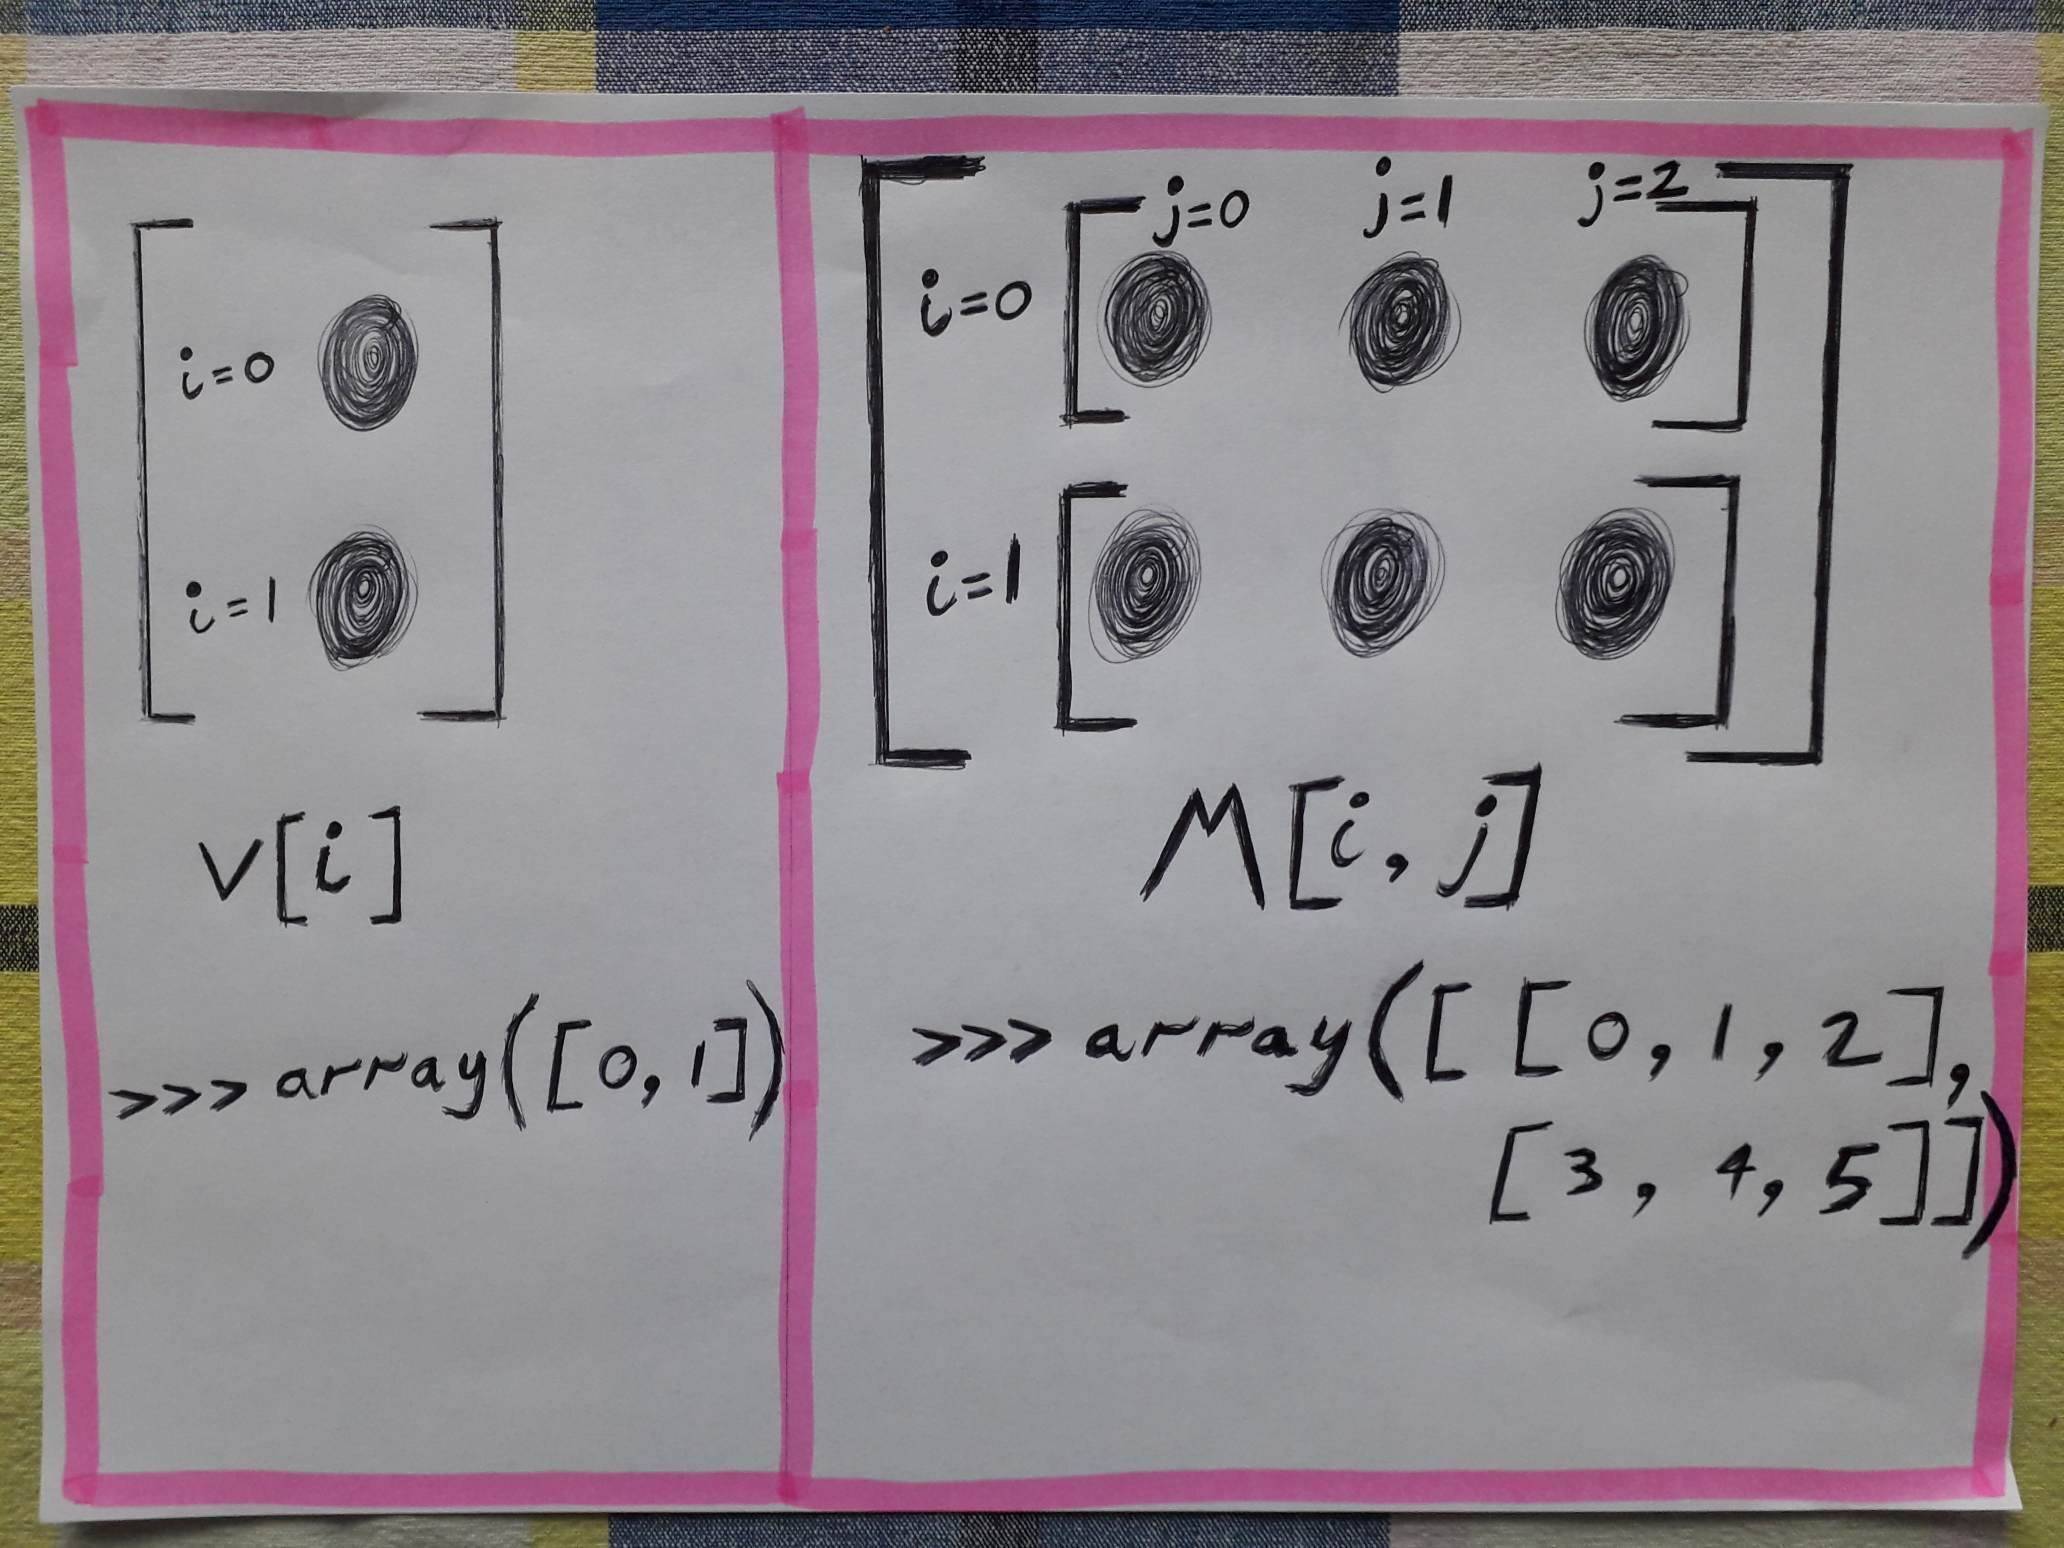
\includegraphics[width=1.00\textwidth]{./images/1d_2d_array.jpg}
\caption{
Visualization of 1D and 2D arrays, respectively.
}
\label{fig:1d_2d_array}
\end{figure}

\newpage
\begin{figure}[ht]
\centering
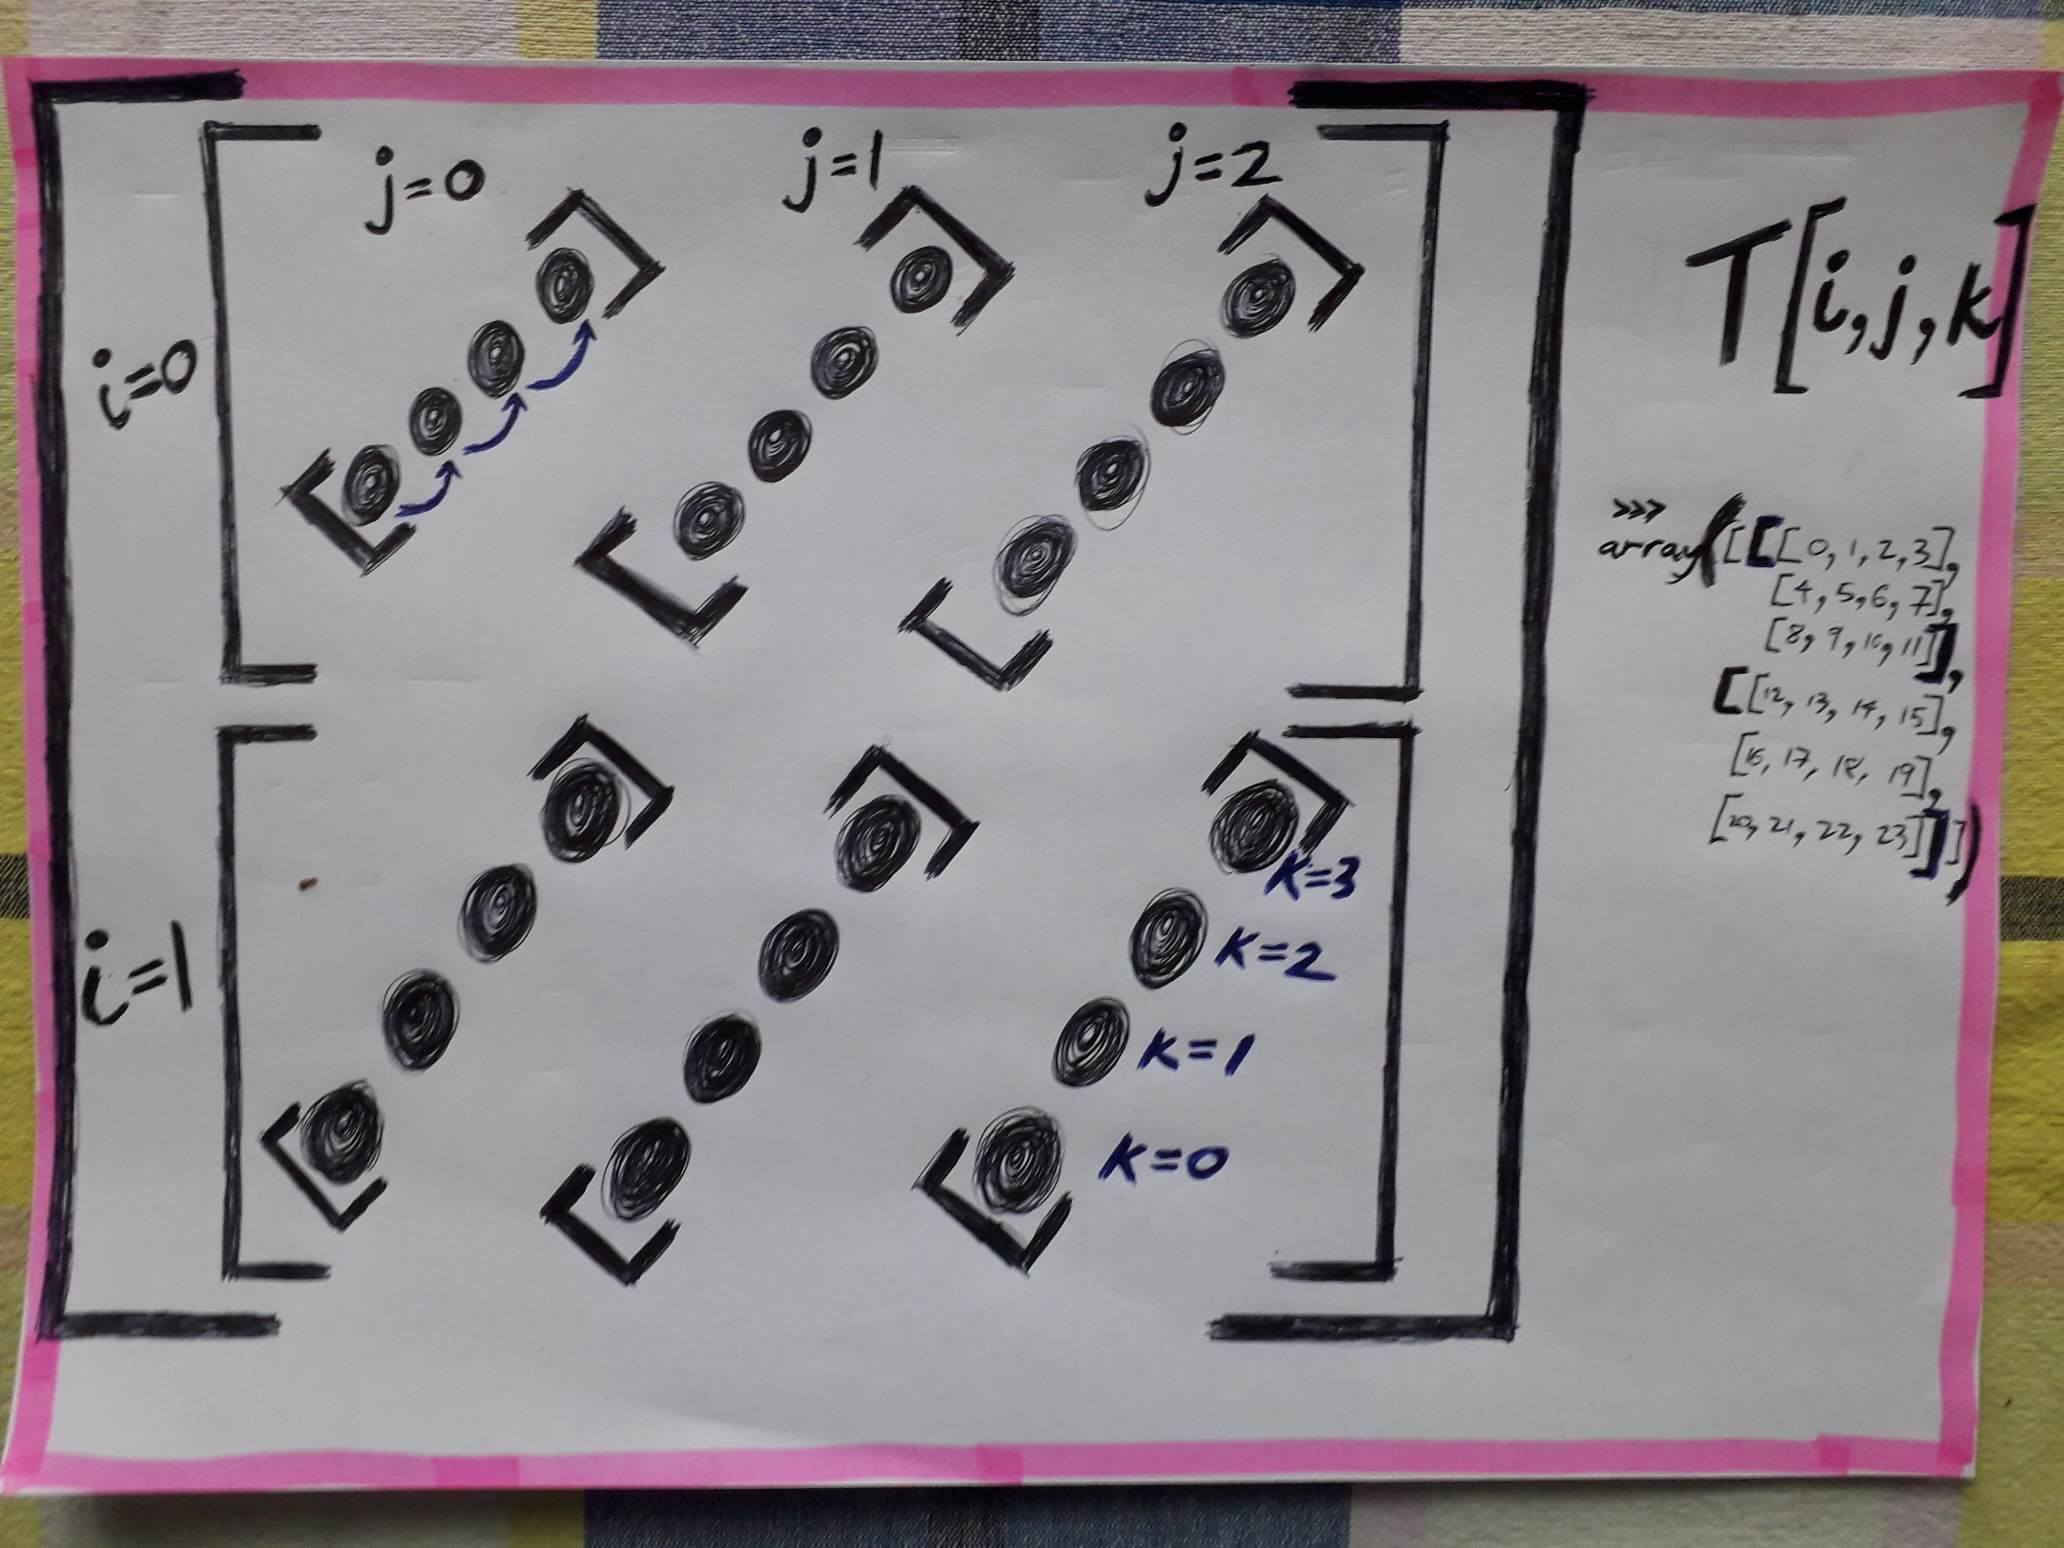
\includegraphics[width=1.00\textwidth]{./images/3d_array.jpg}
\caption{
Visualization of 3D arrays.
}
\label{fig:3d_array}
\end{figure}

\vspace{\baselineskip}
\vspace{\baselineskip}
\vspace{\baselineskip}
\vspace{\baselineskip}

\begin{figure}[ht]
\centering
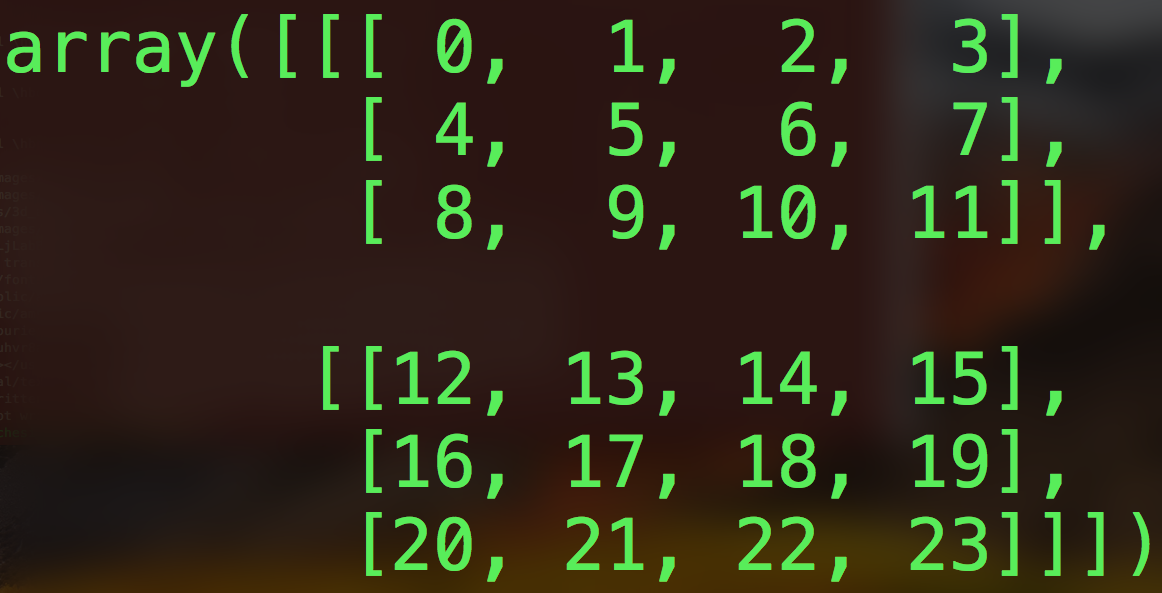
\includegraphics[width=0.65\textwidth]{./images/3d_array_print}
% \caption{
% Visualization of 3D arrays PRINTS.
% }
\label{fig:3d_array_print}
\end{figure}

\newpage